\section{Problema 1: Mutaciones bacteriales}
 
\subsection{Introducci\'on}

El estudio de las mutaciones bacteriales es un trabajo arduo y pesado. 
Una bacteria, al nacer, pertenece a una cepa determinada. 
Con el tiempo, la bacteria va mutando de una cepa a otra hasta que en
alg\'un momento alcanza una cepa terminal desde la cual yo no puede seguir mutando. 
Durante el proceso, estando en una cierta cepa, la bacteria puede mutar hacia algunas otras cepas con una cierta probabilidad;
es decir, no desde cualquier cepa puede mutarse directamente a cualquier otra. 
Afortunadamente, las posibles mutaciones a partir de cada cepa son datos conocidos.
Sin embargo, no se sabe
a priori cu\'anto puede tardar una bacteria en llegar a su estado final. 
Adem\'as, en funci\'on de las posibles mutaciones entre cepas, podr\'ia darse el caso de
que una bacteria que nunca alcance un estado terminal.

Como antecedente para realizar un estudio estad\'istico de este comportamiento, en el cual se estudiar\'an algunas bacterias y para cada una de ellas se registrar\'a cada mutaci\'on ocurrida desde su nacimiento hasta que la misma deja de mutar, se desea predecir si toda sucesi\'on de mutaciones llega a un estado final, y en los casos en los que esto suceda, calcular la sucesi\'on de mutaciones de mayor longitud por la que una bacteria puede
pasar. 

\subsection{Desarrollo}

Comenzamos modelando el escenario del problema como un grafo dirigido (digrafo) donde cada nodo representa una cepa, y cada arista, la mutación de una cepa origen a una cepa destino. 
As\'i, una secuencia de mutaciones equivale a un camino en el digrafo. 
Adem\'as, si el digrafo presenta un ciclo, entonces podemos deducir que existe la posibilidad de que una bacteria nunca alcance una cepa terminal.
Por lo tanto, para resolver el problema planteado, en primer lugar necesitaremos decidir si el digrafo generado es un digrafo ac\'iclico (DAG), y en caso de serlo, encontrar la secuencia m\'as larga de mutaciones equivaldr\'a a hallar el camino (necesariamente simple) m\'as largo dentro de dicho DAG.

Trataremos primero el problema de encontrar el camino simple m\'as largo dentro de un digrafo, suponiendo que este es ac\'iclico. 
Empecemos entonces pensando en como encontrar el camino simple m\'as largo con origen en un nodo cualquiera.
Supongamos que partimos del nodo A. 
El camino m\'as largo que podemos hallar desde A a cualquier otro nodo en el DAG necesariamente
debe pasar por alguno de los nodos sucesores de A. Sea B el nodo sucesor de A tal que el camino m\'as largo con inicio en B es el mayor entre los caminos con inicio en algun nodo sucesor de A:
el camino m\'as largo a partir de A debe ser el camino m\'as largo a partir de B, m\'as la arista que une a A con B.

Esta idea revela una subestructura \'optima sobre la cual tratar el problema (en la secci\'on de Correctiud revisaremos esto). Por otro lado, como varios nodos pueden compartir sucesores, se produce un solapamiento de los subproblemas a resolver.  
Esto nos lleva naturalmente a pensar en aplicar la t\'ecnica de programaci\'on din\'amica en la resoluci\'on del problema.

Definamos, entonces, dado G=(V, E) un DAG, la funci\'on recursiva $F(v)$ como la longitud del camino simple más largo que comienza en el nodo $v$, 

$$F(v)= \max_{(v, u)\;\in\;E} \{F(u)\; + \; 1\}$$

En esta definici\'on consideramos que el m\'aximo de un conjunto vac\'io es 0.

En lugar de implementar una funci\'on recursiva (inmediata a partir de la definici\'on de F), nos centraemos directamente en un
algoritmo iterativo. 
Para esto, debemos entender en que orden debemos resolver los subproblemas, de manera de tener los datos necesarios ya calculados al momento de necesitarlos. 
De la definici\'on de F podemos ver que, al calcular la soluci\'on para un nodo i, solo necesitamos tener las subsoluciones de sus nodos sucesores. 
Para lograr esto, podemos proceder calculando las subsoluciones de los nodos seg\'un un ordenamiento topol\'ogico invertido (es decir, un ordenamiento topol\'ogico recorrido de derecha a izquierda).
Un ordenamiento topol\'ogico de los nodos de un digrafo es aquel en el que ning\'un nodo sucesor aparece antes que su predecesor (es decir, si un digrafo G contiene un eje (u, v), entonces u aparece antes que v en el ordenamiento [Cormen]). Notemos que un digrafo tiene ordenamiento topol\'ogico si y solo si es ac\'iclico, y que este ordenamiento no siempre es único. Por lo tanto, siguiendo el orden propuesto, primero calcularemos los nodos que no tienen sucesores, luego los que tiene como sucesores a los primeros, y as\'i sucesivamente hasta llegar a los nodos que no tienen antecesores.

El algoritmo iterativo de programaci\'on din\'amica mantendr\'a un arreglo $L$, tal que $L[i]$ represente la longitud del camino simple mas largo que nace en el nodo $i$, y lo llenaremos siguiendo el ordenamiento previamente explicado. 
Adem\'as, mantendremos un arreglo $S$, donde $S[i]$ es es el nodo hijo de $i$ que se eligi\'o como subsoluci\'on \'optima al problema de encontrar el camino m\'as largo desde $i$. De esta manera, al terminar el llenado de los arreglos podremos reconstuir el camino simple de mayor longitud que parte de cada nodo.

Calcularemos el ordenamiento topol\'ogico del digrafo siguiendo la idea planteada en [Cormen], el cual propone la utilizaci\'on del algoritmo de recorrido \textbf{DFS} (Depth First Search o búsqueda en profundidad). 
Una ventaja de dicho algoritmo es que procesa digrafo conexos y no conexos sin necesitar hacer distinci\'on, por lo que quedamos exentos de tener decidir si los datos de entrada generan un digrafo de un tipo o del otro. 
Dado que durante la corrida de DFS un nodo $v$ que est\'a siendo explorado aparecer\'a como vecino de alg\'un sucesor $w$ (es decir, $w$ tiene un $back-edge$ a $v$) solo si existe un ciclo, incluimos una verificaci\'on que implica el corte de la ejecuci\'on si un ciclo es detectado, y no afecta al resto de la l\'ogica.
De esta forma, en un \'unico paso inicial decidimos si el digrafo es ac\'iclico mientras que obtenemos la informaci\'on necesaria para proceder con el algoritmo de programaci\'on din\'amica. 

Ahora volvamos al problema original. 
Usando el algoritmo previamente explicado, podemos calcular, para cada nodo $v$, el camino simple m\'as largo que tiene a $v$ como origen.
%Observemos que, de entre todos estos caminos, el de mayor longitud deber\'a tener como primer nodo a alg\'un nodo del DAG cuyo grado de entrada sea cero, y como \'ultimo nodo, alguno cuyo grado de salida sea cero. 
%Para demostrar esto, supongamos un camino simple $C = v_i...v_j$ de longitud m\'axima $n$. 
%Por un lado, si el grado de entrada de $v_i$ es distinto de cero, entonces debe existir alg\'un otro nodo $v_{i-1}$ tal que $v_{i-1}$ no se encuentra en $C$ (por ser el grafo un DAG) y $v_{i-1}$$v_i$ es una arista del digrafo analizado. 
%Pero, siendo este el caso, podr\'iamos agregar tal arista al camino $C$, obteniendo un camino $C' = v_{i-1}v_i...v_j$ de mayor longitud que $C$, lo cual es absurdo pues supusimo $C$ un camino simple de longitud m\'axima.    
%Por otro lado, si el grado de salida de $v_{j}$ es distinto de cero, entonces debe existir alg\'un otro nodo $v_{j+1}$ tal que $v_{j+1}$ no se encuentra en $C$ (por ser el grafo un DAG) y $v_{j}$$v_{j+1}$ es una arista del digrafo analizado. De nuevo, si este el caso, podr\'iamos agregar tal arista al camino $C$, obteniendo un camino $C' = v_i...v_jv_{j+1}$ de mayor longitud que $C$, lo cual es absurdo pues supusimo $C$ un camino simple de longitud m\'axima.
Se desprende que el camino m\'as largo ser\'a el m\'ayor de todas estas soluciones. En el caso en que exista m\'as de un candidato, devolveremos aquel camino que comience en el nodo de menor \'indice. 



\subsection{Algoritmo}
Como ya mencionamos, el algoritmo para generar el orden topol\'ogico est\'a explicado en [Cormen, p603-614]
Las funciones $ordenTopologico$ y $visitar$ consideran a un nodo de la siguiente manera:
ABIERTO, si todavía no se fue visitado; 
DESCUBIERTO, si se lo ha visitado pero todavía no se recorrieron todos sus vecinos;
CERRADO, una vez que se recorrió todos sus vecinos.

Antes de llamar a $ordenTopologico$ todos los nodos son marcados como ABIERTO. 


\begin{algorithm}[H]
\caption{} 
\label{pseudocodigo_ordenTopologico}
\begin{codebox}
\Procname{$\proc{ordenTopologico}(grafo$ G$)$}
\li \While existe nodo ABIERTO en G\Do
\li		n $\gets$ seleccionar nodo ABIERTO
\li		\If visitar(n, nodosOrdenados) igual a HAY CICLO 	\Do 
\li				\Return HAY CICLO
			\End
		\End
\li	\Return nodosOrdenados	  
	\End
\end{codebox}
\end{algorithm}


\begin{algorithm}[H]
\caption{} 
\begin{codebox}
\Procname{$\proc{visitar}(nodo$ n, $lista$ nodosOrdenados$)$}
\li \Comment{El siguiente If es la unica modificacion al algoritmo de Cormen}	
\li \If n es DESCUBIERTO \Do
\li 	 \Return HAY CICLO
 		\End
\li \If n es ABIERTO \Do
\li 	marcar n como DESCUBIERTO
\li		\For cada m sucesor de n \Do
\li			visitar(m)			
			\End	
\li		marcar n como CERRADO
\li 		insertar n al principio de $nodosOrdenados$
\li 	\Return
 		\End
	\End
\end{codebox}
\end{algorithm}
 

\begin{algorithm}[H]
\caption{} 
\label{pseudocodigo_caminoMaximo}
\begin{codebox}
\Procname{$\proc{caminoMaximo}(digrafo$ G$)$}
\li \Comment{ Verificar si hay ciclo en G y obtener orden topologico de sus nodos, si es posible}
\li orden $\gets$ ordentTopologico
\li \If orden es un orden topologico valido (no hay ciclo) \Do
\li		\For cada nodo v en orden invertido\Do
\li			L[v] $\gets$ 0
\li 		S[v] $\gets$ 0
\li			\For cada w sucesor de v \Do
\li		  	\If L[w] + 1 $>$ L[v] \Do
\li				L[v] $\gets$ L[w]+ 1
\li				S[v] $\gets$ w
					\End
				\End
			\End
\li 	camino $\gets$ armarCamino(L, S)
\li 	\Return longitud(camino), camino
		\End
\li \Else \Do
\li 	\Return -1
		\End
	\End
\end{codebox}
\end{algorithm}


\begin{algorithm}[H]
\caption{} 
\label{pseudocodigo_armarCamino}
\begin{codebox}
\Procname{$\proc{armarCamino}(lista$ L , $lista$ S)}
\li camino $\gets$ lista vacia
\li v $\gets$ indice maximo valor en L
\li Agregar v al fin de camino 
\li	\While S[v] distinto de 0 \Do
\li		v $\gets$ S[v]
\li		Agregar v al fin de camino
	\End
\li \Return camino	
	\End
\end{codebox}
\end{algorithm}

\subsubsection{Correctitud} 

Dijimos que el problema presenta un subestructura \'optima. Para ver esto, observemos que la soluci\'on se basa en subsoluciones a subproblemas de igual tipo pero menor tama\~no. 
Podemos afirmar que los tama\~nos de las subinstancias ser\'an menores porque, dado que estamos trabajando sobre un DAG, al tratar de encontrar el camino m\'aximo desde los nodos sucesores de A sabemos que no podemos volver a pasar por A o alguno de sus predecesores puesto que esto implicar\'ia tener un ciclo, lo que no es posible por definici\'on. 
Adem\'as, las subsoluciones deben ser \'optimas: supongamos que tenemos una soluci\'on \'optima que usa una subsoluci\'on no \'optima de un subproblema dado (y que a\'un as\'i la soluci\'on de este subproblema resulta ser la mejor elecci\'on entre las subsoluciones consideradas). Supongamos adem\'as que conocemos una subsoluci\'on \'optima, de manera que el largo de este camino es estrictamente mayor que el de la subsoluci\'on usada. Si reemplazamos, en la soluci\'on, la subsoluci\'on no \'optima por la nueva subsoluci\'on \'optima, entonces obtendremos un camino de mayor longitud que el \'optimo, lo que es absurdo.

Veamos ahora que el algoritmo propuesto calcula el camino m\'as largo. 
Para esto, debemos mostrar que, al finalizar,  el ciclo de las lineas 4 a 10 del Algoritmo \ref{pseudocodigo_caminoMaximo} carga los arreglos $L$ y $S$ de manera que $L[v]$ es la longitud del camino simple m\'as largo desde $v$ a cualquier otro nodo $w$, y que el recorrido generado siguiendo los ejes $(v, S[v])$ (mientras que $S[v]$ est\'e definido) es dicho camino simple. 
Si $v$ no tiene sucesores, entonces no existen caminos de v a ning\'un otro nodo. 
Por lo tanto, $L[v] = 0 = F(v)$ es el valor correcto y no se considera niguna arista ( $(v, S[v]) = (v, indefinido)$ no es un eje existente). 
Si $v$ tiene sucesores, supongamos que los valores de L para estos son correctos (es decir, si $(v, w) \in  E(G)$ entonces $L[w] = F(w)$):
dado que vamos calculando L siguiendo un ordenamiento topol\'ogico le\'ido de derecha a izquierda, los valores de L para los sucesores de v ya habr\'an sido calculados al momento de llegar a $v$. 
Como ya vimos, para llegar a cualquier nodo alcanzable desde $v$ debemos pasar por alguno de los sucesores de $v$.  Entonces, la distancia maxima de $v$ a cualquier otro nodo depende de la distancia m\'axima de sus sucesores a cualquier otro nodo: en el algoritmo, el subciclo de las lineas 7-10 elige el sucesor $w$ con mayor $L[w]$ y se guarda $w$ en $S[v]$. Asi, $L[v] = \max_{(v,w) \in E(G)}{L[w]+1} = \max_{(v,w) \in E(G)}{F(w) +1} = F(v) $
El recorrido $vS[v]S[S[v]]...S[...S[v]]...0$ es un camino simple, pues al ser el digrafo ac\'iclico, ning\'un nodo puede tener como sucesor a alguno de los anteriores.


\subsubsection{An\'alisis de complejidad}
 
El Algoritmo \ref{pseudocodigo_ordenTopologico}, al ser \textbf{DFS}, tiene orden O($\left|{E}\right|$+$\left|{V}\right|$).
El Algoritmo \ref{pseudocodigo_armarCamino} recorre un arreglo con O($\left|{V}\right|$) posiciones, y dado que se asume que no existen ciclos, a lo sumo pasa una vez por cada posici\'on. Por lo tanto, es del orden O$\left|{V}\right|$).
En el Algoritmo \ref{pseudocodigo_caminoMaximo} se recorren todos los nodos del grafo una \'unica vez (en el ciclo de las l\'ineas 4-12), y por cada uno, se recorren todas sus aristas tambien una \'unica vez (en el ciclo de las l\'ineas 7-10), por lo que el el ciclo mayor tiene complejidad en el orden de O($\left|{E}\right|$+$\left|{V}\right|$). Adem\'as, se llama a cada una de las dos funciones previamente mencionadas una \'unica vez: en total, la complejidad del algoritmo resulta en el orden de O($\left|{E}\right|$+$\left|{V}\right|$).
 

\subsection{Pruebas}
Para las pruebas de correctitud utilizamos grafos peque\~nos que pueden resolverse f\'acilmente a mano. 
Los casos que elegimos fueron digrafos con ciclos y sin ciclos, tanto de una \'unica componente conexa como m\'as de una.


Para probar la performance del algoritmo, armamos casos de digrafos aleatorios (que pueden o no contener ciclos) y DAGs. Probamos casos separados por n\'umero de nodos fijos (sobre los que variamos la cantidad de aristas) y n\'umero de aristas fijo (donde variamos la cantidad de nodos). 
No encontramos familias de casos que tuvieran un comportamiento distinto al esperado.

%%%%%%%%%%%%%%%%%%%%%%%%%%%%%%%%%%%%%%%%%%%%%%%%%%%%%%%%%%%

\begin{figure}[H]
	\centering
	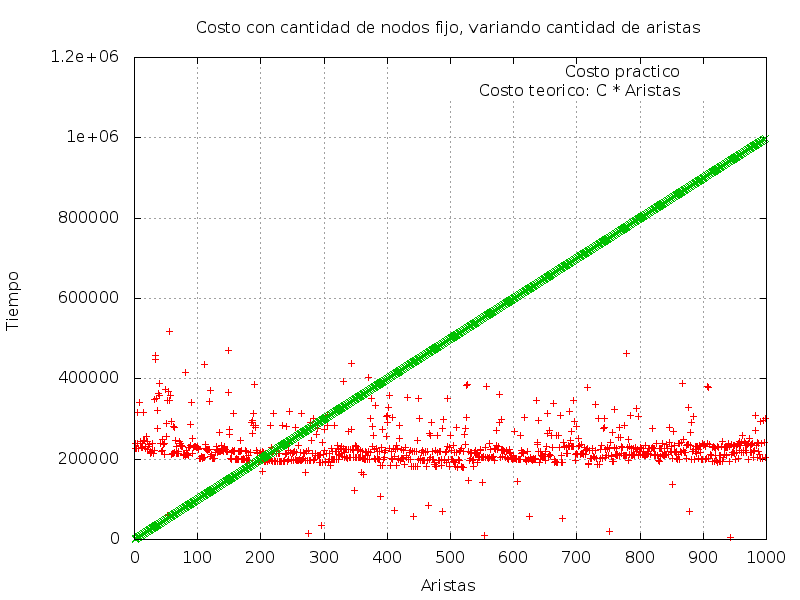
\includegraphics[scale=0.5]{dag_100.png}
	\caption{Digrafo aleatorio, n = 100, m variable}
\end{figure}

\begin{figure}[H]
	\centering
	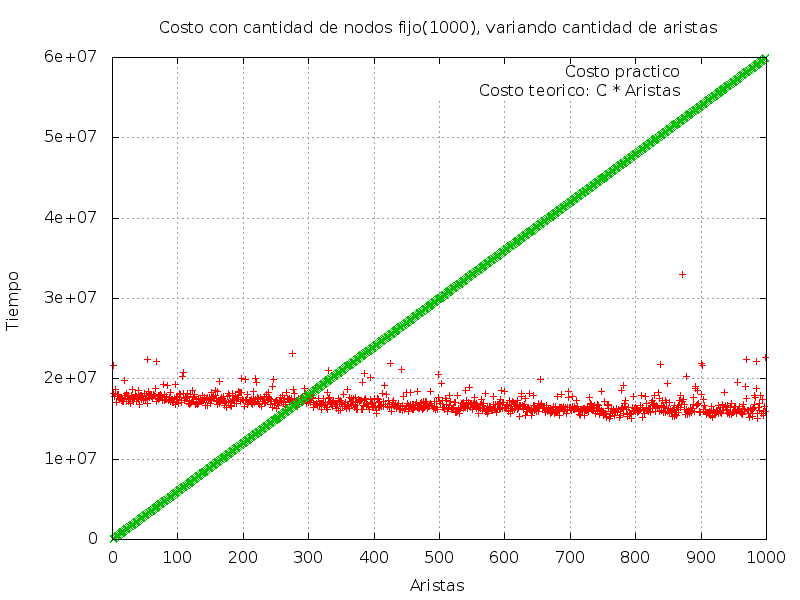
\includegraphics[scale=0.5]{dag_1000.png}
	\caption{Digrafo aleatorio, n = 1000, m variable}
\end{figure}


%%%%%%%%%%%%%%%%%%%%%%%%%%%%%%%%%%%%%%%%%%%%%%%%%%%%%%%%%%%

\begin{figure}[H]
	\centering
	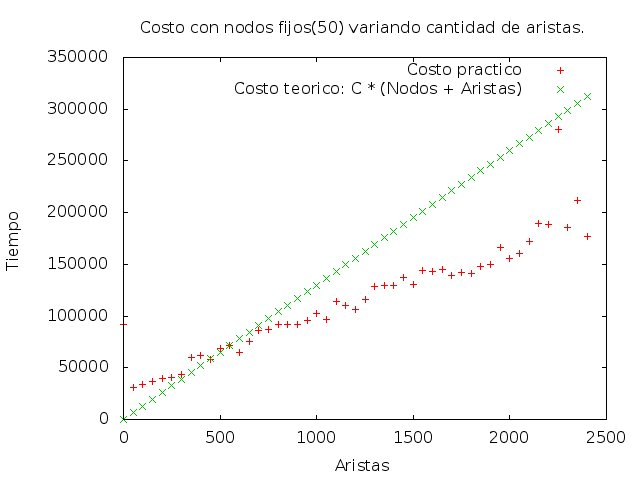
\includegraphics[scale=0.5]{blank.png}
	\caption{DAG aleatorio, n = 100, m variable}
\end{figure}

\begin{figure}[H]
	\centering
	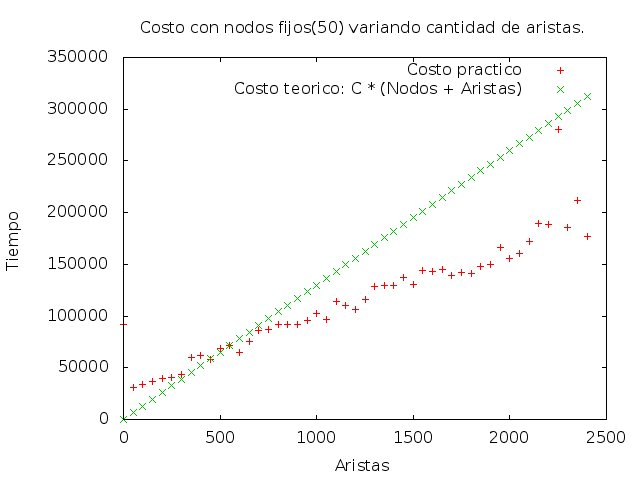
\includegraphics[scale=0.5]{blank.png}
	\caption{DAG aleatorio, n = 1000, m variable}
\end{figure}

%%%%%%%%%%%%%%%%%%%%%%%%%%%%%%%%%%%%%%%%%%%%%%%%%%%%%%%%%%%

\begin{figure}[H]
	\centering
	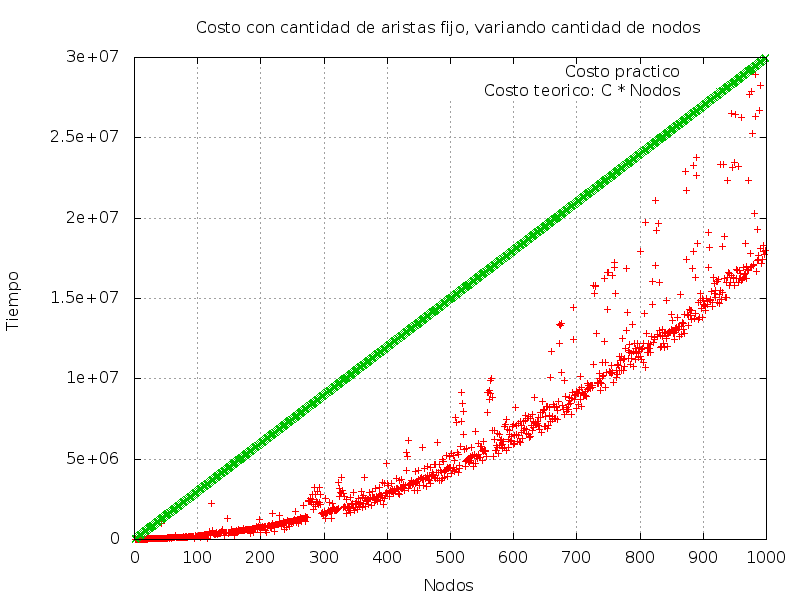
\includegraphics[scale=0.5]{dag_100_n_var.png}
	\caption{Digrafo aleatorio,  n variable, m = 100}
\end{figure}

\begin{figure}[H]
	\centering
	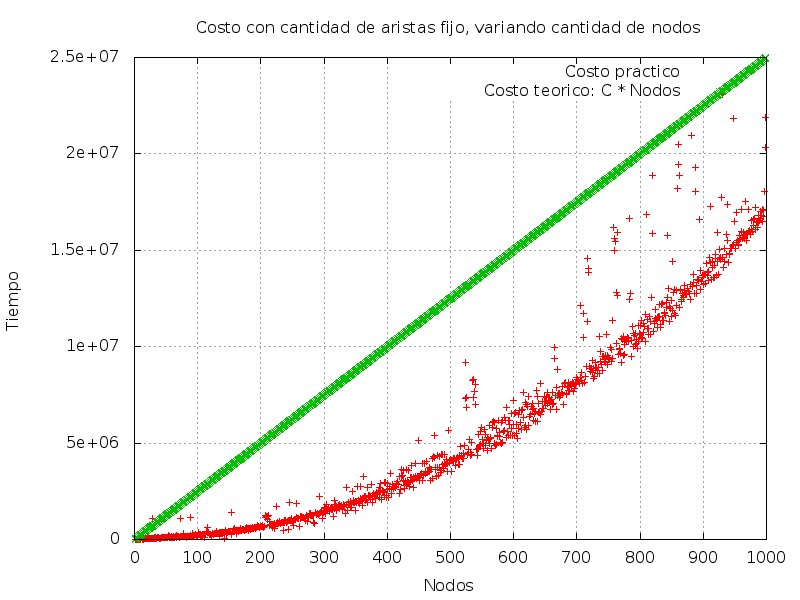
\includegraphics[scale=0.5]{dag_500_n_var.png}
	\caption{Digrafo aleatorio, n variable, m = 500}
\end{figure}



%%%%%%%%%%%%%%%%%%%%%%%%%%%%%%%%%%%%%%%%%%%%%%%%%%%%%%%%%%%

\begin{figure}[H]
	\centering
	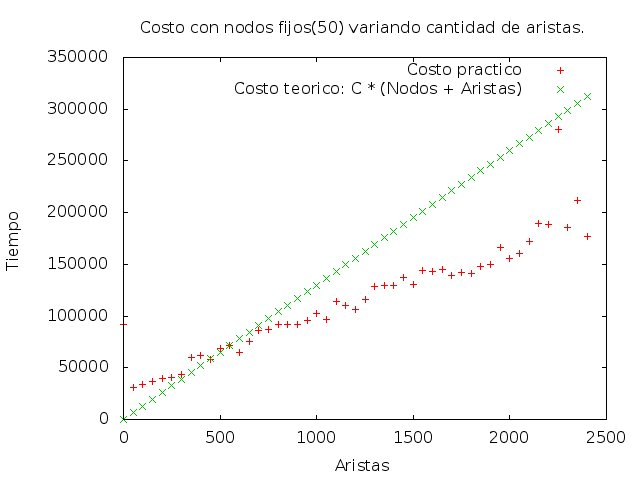
\includegraphics[scale=0.5]{blank.png}
	\caption{DAG aleatorio,  n variable, m = 100}
\end{figure}

\begin{figure}[H]
	\centering
	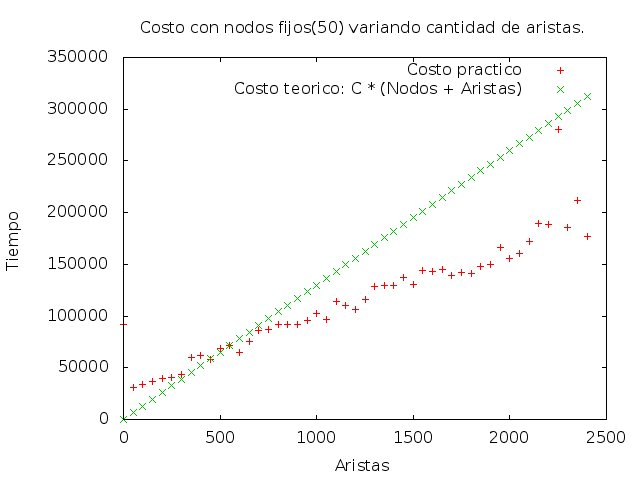
\includegraphics[scale=0.5]{blank.png}
	\caption{DAG aleatorio, n variable, m = 500}
\end{figure}


%%%%%%%%%%%%%%%%%%%%%%%%%%%%%%%%%%%%%%%%%%%%%%%%%%%%%%%%%%%

\subsection{Conclusiones}

La resoluci\'on del problema planteado en este ejercicio es un claro ejemplo de la importancia de t\'ecnicas como Programaci\'on din\'amica y algoritmos gen\'ericos sobre grafos: no solo se obtuvo un algoritmo competente en cuanto a performance (por ser de orden lineal tanto en tiempo de ejecucion como almacenaiento de datos en memoria), sino que tambien resulta ser sencillo y f\'acil de comprender.

Los resultados de los test con n\'umero de nodos fijos y n\'umero de arista variables no fueron los experados; a pesar de no contradwecir la complejidad calculada, esperabamos ver un comportamiento lineal, m\'as que el aparente comportamiento constante. No pudimos dilucidar el origen de hecho.
A pesar de no estar presentes, hubiera sido interesante agregar casos de test donde variasemos la cantidad de componente conexas dejando fijas la cantidad de nodo y aristas, o la suma de ambos valores. En este caso, esperariamos que el grafico estuviera acotado por una funci\'on constante.

